%%%%%%%%%%%%%%%%%%%%%%%%%%%%%%%%%%%%%%%%%%%%%%%%%%%%%%%%%%%%%%%%%%%%%%%%%%%%
%                        message-authentication.tex                        %
%%%%%%%%%%%%%%%%%%%%%%%%%%%%%%%%%%%%%%%%%%%%%%%%%%%%%%%%%%%%%%%%%%%%%%%%%%%%

\section{HMAC-SHA-1}

For the request authentication portion of the feedback API, we're using the HMAC SHA-1
algorithm. The algorithm works as follows. The client and server share a secret key.
Whenever the client sends a request to the server they compute the SHA-1 hash value of
a certain portion of the request using the secret key and they include that hash value
as one of the request headers. When the server receives a request, they use the same
algorithm to compute what the hash value for the request should be. If the expected hash
doesn't match the hash sent in the request then the authentication step fails, otherwise
it passes. The hash values will be different if either the secret key is not the same
for both sides, or the algorithm is not exactly the same. Here is an image that depicts
the algorithm:

\vspace{1cm}

\begin{center}
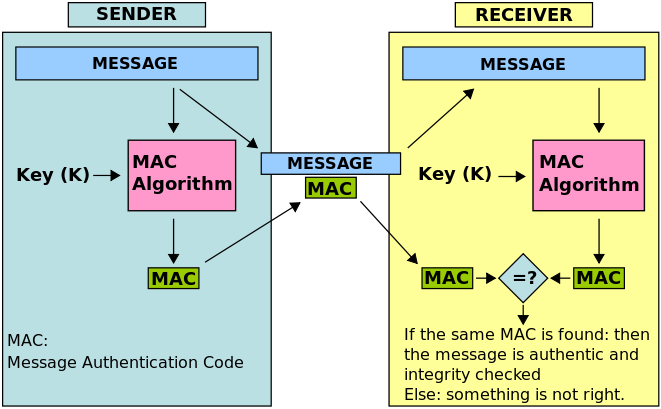
\includegraphics[width=0.8\textwidth]{HMAC_Explanation.png}
\end{center}


%%%%%%%%%%%%%%%%%%%%%%%%%%%%%%%%%%%%%%%%%%%%%%%%%%%%%%%%%%%%%%%%%%%%%%%%%%%%

\section{How to Sign a Request}

For all requests, the server expects to find the request signature in the \\
\textbf{\textit{Feedback-Component-HMAC-SHA-1~}}
header variable.

\subsection{GET and DELETE Requests}

For GET and DELETE requests, the hash value is computed from the concatenation
of the http verb, resource path, and query string in that order.
\subsubsection{Examples}

For the following examples assume that the secret key is the string 'secret key'.

\begin{center}
\begin{tabular}{|l||l|}

\hline
\multicolumn{2}{|c|}{\textbf{Get Feedback List}} \\
\hline
\textbf{HTTP Verb}                  & GET \\
\hline
\textbf{Resource Path}              & /ichiba/win8/feedback \\
\hline
\textbf{Query}                      & ?minScore=3 \\
\hline
\textbf{Data that should be Hashed} & GET/ichiba/win8/feedback?minScore=3 \\
\hline
\textbf{Hash Signature}             & 81e5913c6757e03d4db7af14bc9dff44a0deca95 \\
\hline

\end{tabular}
\end{center}

\subsection{POST and PUT Requests}
For POST and PUT requests the hash value is computed from the concatenation
of the http verb, resource path, query, and request body in that order.

\subsubsection{Examples}

\begin{center}
\begin{tabular}{|l||l|}

\hline
\multicolumn{2}{|c|}{\textbf{Create Feedback Record}} \\
\hline
\textbf{HTTP Verb}                  & POST \\
\hline
\textbf{Resource Path}              & /ichiba/win8/feedback \\
\hline
\textbf{Query}                      & N/A \\
\hline
\textbf{Body}                       & \{"hello":"world"\} \\
\hline
\textbf{Data that should be Hashed} & POST/ichiba/win8/feedback\{"hello":"world"\} \\
\hline
\textbf{Hash Signature}             & 0a5cb6a2c36c713dfbd57777c751807f5233f481 \\
\hline

\end{tabular}
\end{center}

\begin{center}
\begin{tabular}{|l||l|}

\hline
\multicolumn{2}{|c|}{\textbf{Create User}} \\
\hline
\textbf{HTTP Verb}                  & POST \\
\hline
\textbf{Resource Path}              & /ichiba/win8/users \\
\hline
\textbf{Query}                      & N/A \\
\hline
\textbf{Body}                       & \{\} \\
\hline
\textbf{Data that should be Hashed} & POST/ichiba/win8/users\{\} \\
\hline
\textbf{Hash Signature}             & c94d478f159ba92ca55e51595e95006e8e088ca2 \\
\hline

\end{tabular}
\end{center}

